% DO NOT REMOVE -- This fixes issues where Acrobat on Windows cannot open PDFs
\pdfminorversion=4

% Change to use the correct class file for your paper.
\documentclass[10pt,preprint,abstract]{sensys-proc}

%\pagenumbering{arabic}

%\usepackage{adjustbox}    % Auto-resize table content (eg Opo SenSys'14 rel)
\usepackage{amsfonts}     % Adds math fonts, commands such as \begin{align}
\usepackage{array}        % Tables for use in math mode
\usepackage{booktabs}     % Elegant table-formatting library
\usepackage{bold-extra}   % Provides bf+sc (only in textbf+textsc env.)
\usepackage{bytefield}    % Formatting and layout of packets / bytefields
\usepackage[skip=5pt]{caption}
\usepackage[sort,nocompress]{cite} % sort citations
\usepackage{colortbl}     % Color table cells
\usepackage{comment}      % Provides \begin,\end{comment} for large blocks
\usepackage{cprotect}     % Allows verbatim, other formatting in macro args
\usepackage[ampersand]{easylist} % Simpler list syntax
\usepackage{endnotes}     % Footnotes pushed to the end of a document
\usepackage{gensymb}      % Adds useful symbols w/out math mode, e.g. \degree
\usepackage{graphicx}     % For importing graphics
\usepackage{lipsum}       % For generating temporary filler text
\usepackage{listings}     % in-line source code (poorly, consider minted)
\usepackage{mathtools}    % amsmath extension, adds more math formatting
\usepackage[protrusion=true,expansion=true,kerning,spacing]{microtype} % better type, spacing
\usepackage{multirow}     % Multiple row spacing in tables
\usepackage{nth}          % Typeset 33rd correctly as \nth{33}
%\usepackage[section]{placeins} % Don't let figs escape their sections
\usepackage{rotating}     % Rotates any object, note sideways != sidewaysfigure
%\usepackage[all=normal]{savetrees} % For when space is tight, read manual and
                          % selectively enable things. CAN BREAK CONF STYLES!!
\usepackage{soul}         % Provides \hl{} for highlighting
%\usepackage{subfig}
%\usepackage{subfigure}    % Complicated figure creation
\usepackage[subrefformat=parens]{subcaption}   % Replaces both subfig and subfigure
\usepackage{tabularx}     % Complicated table creation
\usepackage{textcomp}     % Provides \textmu for upright mu's
\usepackage{threeparttable} % Add footnotes to a table
%\usepackage{times}        % Force use of the Times font
\usepackage{units}        % For nice fractions, \nicefrac{1}{2} --> 1/2
\usepackage{url}          % Pretty printing of hyperlinks
\usepackage[usenames,dvipsnames,svgnames]{xcolor} % Allow the use and definition of colors
\usepackage{xspace}       % Intelligently add spaces after commands

% The hyperref package must loaded last. Can conflict with some packages, see:
% README ( http://ctan.mackichan.com/macros/latex/contrib/hyperref/README.pdf )
\usepackage[colorlinks=true,citecolor=violet,urlcolor=blue]{hyperref}     % Creates hyperlinks from ref/cite
\hypersetup{pdfstartview=FitH} % Sets default zoom to 100% width

% And, of course, cleveref must be loaded last-last (read: after hyperref)
\usepackage[capitalise,nameinlink,noabbrev]{cleveref}     % Do the right thing with fig/table references

\DeclareCaptionType{copyrightbox}

\newlength\SUBSIZE

\renewcommand{\arraystretch}{1.2} % Space out rows in tables

% Break URLs properly (thanks to Alex Halderman)
\def\UrlBreaks{\do-\do\.\do\@\do\\\do\!\do\_\do\|\do\;\do\>\do\]\do\)\do\,\do\?\do\'\do+\do\=\do\#}
\def\UrlBigBreaks{\do\:\do\/}

% Don't typset URLs in tt font
\urlstyle{same}

%\setlength\paperheight {11in}
%\setlength\paperwidth {8.5in}

% Set the graphics path
\graphicspath{{../figs/}{../images/}}


% No space between bibliography items:
\let\oldthebibliography=\thebibliography
  \let\endoldthebibliography=\endthebibliography
  \renewenvironment{thebibliography}[1]{%
    \begin{oldthebibliography}{#1}%
      \setlength{\parskip}{0ex}%
      \setlength{\itemsep}{0ex}%
  }%
  {%
    \end{oldthebibliography}%
  }

% Tighten up paragraph indents
%\setlength{\parindent}{5mm}

% Some macros that a broadly useful:
\newcommand{\uW}{{\textmu}W\xspace}
\newcommand{\uA}{{\textmu}A\xspace}
\newcommand{\um}{{\textmu}m\xspace}
\newcommand{\us}{{\textmu}s\xspace}
\newcommand{\uF}{{\textmu}F\xspace}
\newcommand{\uJ}{{\textmu}J\xspace}
\newcommand{\iic}{I$^2$C\xspace}

\newcommand{\nameos}{Tock\xspace}
\newcommand{\namedevice}{Storm\xspace}

\definecolor{light-gray}{gray}{0.75}
\newcommand{\glipsum}[1][1]{
  \textcolor{light-gray}{\lipsum[#1]}
}

\begin{document}

\title{Poster Abstract: A Networked Embedded System Platform for the Post-Mote Era}

%% % AUTHOR STYLE 1
%% \author{
%%  \alignauthor{Author 1, Author 2, and Author 3}\\
%%  \affaddr{Electrical Engineering and Computer Science Department}\\
%%  \affaddr{University of Michigan}\\
%%  \affaddr{Ann Arbor, MI 48109}\\
%%  \email{\{uniqname1,uniqname2,uniqname3\}@umich.edu}
%% }

% AUTHOR STYLE 2
\author{
\begin{tabular}{ccc}
  \multicolumn{3}{c}{
    Pat Pannuto$^\dagger$,
    Michael P Andersen$^\ddagger$,
    Tom Bauer$^\S$,
    Bradford Campbell$^\dagger$,
    Amit Levy$^\S$,
  } \\
  \multicolumn{3}{c}{
    David Culler$^\ddagger$,
    Philip Levis$^\S$,
    and
    Prabal Dutta$^\dagger$
    \vspace{0.3cm}
  } \\
  %
  \affaddr{$^\dagger$Computer Science \& Engineering} &
  \affaddr{$^\ddagger$Computer Science \& Engineering} &
  \affaddr{$^\S$Computer Science \& Engineering} \\
  %
  \affaddr{University of Michigan} &
  \affaddr{University of California, Berkeley} &
  \affaddr{Stanford University} \\
  %
  \affaddr{Ann Arbor, MI 48109} &
  \affaddr{Berkeley, CA 94720} &
  \affaddr{Stanford, CA 94305} \\
  %
  \affaddr{\{ppannuto,bradjc,prabal\}@umich.edu} &
  \affaddr{\{m.andersen,culler\}@berkeley.edu} &
  \affaddr{\{tbauer01,levya,pal\}@stanford.edu} \\
\end{tabular}
}

% Michael Andersen <m.andersen@eecs.berkeley.edu> 
% Patrick Pannuto <ppannuto@umich.edu> 
% Brad Campbell <bradjc@umich.edu> 
% Amit Levy <levya@cs.stanford.edu> 
% Tom Bauer <tbauer01@stanford.edu> 
% Philip Levis <pal@cs.stanford.edu> 
% Prabal Dutta <prabal@eecs.umich.edu> 
% David Culler <culler@berkeley.edu> 

\crdata{978-1-4503-3143-2/14/11}
\doidata{10.1145/2668332.2668364}
\conferenceinfo{SenSys'14,} {November 3--6, 2014, Memphis, TN, USA.}

\maketitle

\begin{abstract}
% ABSTRACT

Write abstract here.
Header information is handled by \LaTeX{} magic.


\end{abstract}

% \category{B.4.2}{HARDWARE}{Input/Output and Data
%   Communications}[Input/Output Devices]
% \category{C.3}{COM\-PU\-TER-COM\-MU\-NICATION
%   NET\-WORKS}{Spe\-cial-Purpose and App\-li\-cation-Based Systems}
% \terms{Design, Experimentation, Measurement, Performance}
% \keywords{Mobile phones, Energy harvesting, Phone peripherals, Audio
%   communications, Participatory sensing}

%% SUBMISSION INSTRUCTIONS
%% Posters must be submitted as a single PDF containing no more than 3 pages. The
%% first two pages should contain an abstract describing the research content of
%% the poster, along with title, authors, institutional affiliations and contact
%% information. The third page should contain a thumbnail draft of the poster’s
%% contents.

% page limit          % 2
% abstract            % 0.5 pg
%\vfill\eject
\section{Introduction}
\label{sec:intro}

Over a decade ago, a flurry of hardware platforms and supporting software
empowered the research community to investigate and explore wireless sensor
networks and their applications. Many papers today still use these
``mote''-class devices, exploring problems in systems software, low-power
networking, and application design.

The underlying technology and its potential applications have progressed a
great deal in the past ten years. The Cortex~M series of 32-bit processors
finally have sleep currents competitive with MSP430 and AVR microcontrollers.
802.15.4 has grown far beyond the destructively closed world of ZigBee, with
new physical layers for new applications. The recent incorporation of
Bluetooth Low Energy (BLE) into mobile phones allows ubiquitous sensing networks to
directly interact with human-centric devices. Also driven by phones, sensors
themselves are orders of magnitude more energy efficient and precise.

Simultaneously, applications have become much richer. Applications in early
sensor network research focused on fixed rate, long-term sensing, guiding a
research agenda of ultra-low power operation and robust multi-hop networking.
Today, personal area networks, tethered to a phone, interact with
proximity networks through iBeacon; intra-vehicle networks connect speakers
and microphones to a phone; building-area networks share knowledge, like
occupancy, among security, HVAC, and lighting monitoring and control.

We have an explosion of new applications, each with new and challenging
requirements. We have reached a turning point in hardware, enabling a whole
new class of device and operational models. It is time for a new platform to
explore and research embedded networked systems in the post-mote era.

         % 0.5 pg
\section{Technology Today}
Advancements in three major areas---networking, MCUs, and energy
harvesting---open new opportunites for networked embedded systems and generate
new implications on how an OS should manage activity, security, and privacy.

%  Need a sentence in 2 that explains what BLE is/why it's important. I.e.,
%  iBeacon, it's how mobile devices are going to interact with ubiquitous
%  computing/proximity sensor networks. Lower power than 802.15.4, etc. There is
%  no explanation of what it is, instead it jumps to TinyOS considerations.

\smallskip\noindent
\textbf{Integrating TinyOS and Bluetooth Low Energy.}
BLE provides highly efficient beaconing,
bidirectional communication, fast device discovery, authentication, and
optional pico-network formation and management~\cite{ble-overview}.
BLE explicitly incoporates ideas of periodic beacons and duty cycles,
such that a device with a wakeup latency of a second can have
an average current draw of $< 40$~\uA.\footnote{
  e.g. Nordic Semiconductor NRF8001.
}
%
Tight timing requirements mean that most chips have tightly
integrated software stacks that present limited abstractions such as
getting and setting attributes. Furthermore, these software stacks
assume a threaded, sequential execution model that in our experience
is hard to adapt efficiently to an event-driven paradigm. Integrating an
event-driven OS with manufacturer-provided software is a
challenge that a post-mote platform must address.

% The question remains open whether a sequential
% system with the same versatility as TinyOS could eliminate these
% inefficiencies.  Also, it is possible that a stack
% constructed from the ground up that leveraged event driven programming and BLE
% technology could result in an embedded system more efficient than the
% manufacturer provided software implementations.  BLE is an excellent
% technology to be used in embedded systems but integrating TinyOS with stacks
% provided by manufactures is not sustainable nor ideal for future research.

\smallskip\noindent
\textbf{Cortex M0--M4.}
Advancement in MCU technology has widened the field of low-power processors
which now ranges from highly performant cores such as the 1~\uA--30~mA,
0.5--120~MHz Atmel SAM4S with a Cortex~M4, 2~MB flash, and 160~kB SRAM to
highly efficient cores such as the 5~nW--10~\uA, 1--8~MHz M3 research
chips~\cite{lee13modular} with a Cortex~M0 and 16~kB of memory.
%
While the ultra-low power M3 resembles traditional embedded MCUs, for
the cm-scale domain powerful primitives such as memory management and dynamic
frequency scaling are becoming available.
To still meet low power targets, however, these MCUs have very complex power
management and peripheral configuration mechanisms.
The post-mote OS will need to devise new means to efficiently abstract %(near)
optimal power management for these more complex chips and leverage the new
features when available without sacrificing its utility for less feature-rich,
constrained systems.

% While these are fairly
% easy to configure and abstract if energy usage is not a concern, as in most
% Arduino-type systems, optimal energy usage requires a very close coupling
% between dynamically changing application states and peripheral configurations.

% Interesting and fair point, but more on the systems side than the MCU, which
% is the discussion here (and we only have 2 pages..)
%
% A final characteristic is that the increase in DMA channels combined with the
% ability to configure peripheral events to asynchronously trigger other
% peripherals and DMA transfers allows experienced programmers to implement
% important parts of application logic with no CPU cycles - which can
% drastically reduce the time that the CPU is spent awake. The configuration of
% such functionality is fairly hardware specific and the question of how to
% automatically use this functionality or present it to novice programmers in an
% easy to use form is challenging.

\smallskip\noindent
\textbf{Impact of Energy Harvesting.}
%Today, it is possible to obtain temperature, humidity, or light levels every
%minute or two, under dimly lit conditions, using indoor photovoltaics that
%occupy a mere 2--3~cm$^2$.
%
%It is possible to build an energy-harvesting energy meter that measures
%real power in a form factor no larger than a clip-on split-core current
%transformer.
%
A decade of research in energy-harvesting transducers, efficient power
electronics, and compact energy storage technologies, coupled
with reductions in the idle and active power of radios,
instant-on/instant-write phase-change memory, and the efficacy of modern MCUs
make compact energy-harvesting sensors that can run perpetually, even in
indoor settings, a reality~\cite{doubledip}.
%
However, writing applications for intermittently-powered,
energy-harvesting systems is a challenge.  It requires revisiting many
assumptions about system startup, maintaining state across activation cycles,
discovering and communicating with neighbors, predicting future energy
availability, and scheduling operations under energy uncertainty~\cite{dewdrop}.
%
Deriving clearer power state and availability semantics, and a means to express
what state needs to be saved, present new embedded OS challenges.

%One way to
%circumvent some of the challenges is to grossly over provision the energy
%harvesting power supply in an attempt to mask the energy intermittency and all
%that dealing with it entails.  But this drives up size and cost, and it cannot
%fully mitigate the variability inherent in energy-harvesting operation.  A
%different path exposes the variability, perhaps through richer power supply
%interfaces, to the system software which can then context switch on time or
%energy quanta, and manage continuations across activations by leveraging fast
%and efficient context storage and restoration.


\section{Applications Today}

A decade ago, stationary fixed rate (or occasionally event-driven) data 
reporting applications dominated sensor networks and their research. 
New applications that incorporate mobility, hybrid networking, and 
personal privacy are emerging. A new platform should embrace and enable 
these new opportunities.

\subsection{Human-centric}

The mobile device is a gateway to an embedded networks. Instead of
sending data to a fixed collection point, the network can send directly
to a mobile device, on demand. This enables a person to interact with
the surrounding devices and infrastructure without needing to know a
URL or log into a cloud-based system. Proximity networks provide a degree
of basic, physical security that enables such opportunistic interactions.
Consider the venerable sensor network example of conference rooms. 
Rather than go through a web page or other centralized application, 
you can walk into a room and directly control its lights. 
A data collection gateway for room occupancy,  in addition to streaming
data for durable storage and offline analysis, can make that data
available to your device directly. You can walk into a room, turn on its 
lights, ask it how long it is free for, and see what other rooms are free.

Because these interactions are human-centric, they require low latency and
are highly bursty -- two performance properties unimportant in the 
dominant network model of the past decade. These low-latency interactions
are more than event notifications or alarms. They can involve significant
queries and exchanges of data. Furthermore, becuase they involve mobile
devices, existing approaches of long-term link estimation are of limited use.
These new application requirements will force us to rethink the tradeoffs
between latency, storage, energy, snooping, and how an operating system will
support them.

\subsection{Perpetual Networks}

Energy harvesting and low-power peripherals will finally enable a
long-term goal of the sensor network community: perpetual networks. Imagine
an iBeacon that, once installed, could possibly run forever. Or smoke detectors that need no battery replacements. If the world will be filled with
thousands of smart objects per person, energy must recede to be a non-issue
for almost all of them.

We still can't predict the weather, and so we of course also still can't 
predict the performance of a solar cell. This means an operating system
is stuck between two big unknowns: the future energy available as well as
the potential energy needs from bursty, human-centric interactions. For
an embedded device to be truly perpetual, it must scale its behavior and
perfomance based on these two factors, optimizing how it uses its energy
as needed. 


\sub


\smallskip\noindent
\textbf{How Applications Drive Platforms.}

\glipsum[1]

\smallskip\noindent
\textbf{Privacy and Proximity in Networks.}
Interactions between PANs (centered around a user’s mobile phone)
and proximity applications such as iBeacons happen in public, with
never-seen-before peers. This presents a dual security and privacy problem. On
the one hand, connections between the PAN and proximity device must be
confidential and authentic -- e.g. payments.
On the other hand, casual interactions with
proximity devices must not enable ubiquitous tracking of users. Unfortunately,
confidential and authentic communication and anonymity are difficult to
achieve simultaneously.
%
Operating systems can play a role in addressing these issues, for example by coordinating
security features in the BLE stack with application specific knowledge.

%% Too detailed an example for a poster abstract
%
% For example, we propose a new mechanism -- Address Isolation -- that leverages
% Resolvable Private Addresses in BLE to expose multiple private identities from
% the same end-user device. Resolable Private Addresses are BLE device addresses
% derived from a public random value and a shared secret between peers. This
% allows peers to identify each other through addresses that appear random to
% nearby devices that do not share the secret. Address Isolation uses this BLE
% mechanism to expose multiple identities (each resolvable by, e.g. a single
% point-of-sale operator, but anonymous to everyone else) at the OS level, by
% coordinating when each identity should be used with applications. For example,
% in the point-of-sale scenario, the application loads a shared secret key with
% a point-of-sale operator (e.g. Wal-Mart) at application install time, and
% tells the operating system to use the identity based on that key upon user
% interaction, such as initiating a payment.


\section{A New Platform, Hardware and Software}

To begin, we design two complementary hardware platforms. First, \namedevice,
a full-featured platform with a Cortex~M4 processor with many advanced
features (memory protection, DSP instructions) to explore novel embedded OS
concepts, 802.15.4 and BLE radios to support connectivity with both
established low-power wireless technology and emerging PANs, and a highly
instrumented and flexible power network to enable fine-grained measurement and
control. Second, Squall, a price and area-optimized platform for massive
dissemination and large-scale testing with BLE connectivity that leverages an
integrated SoC Cortex~M0 for computation.

The increased complexity of peripherals, power management, and clock
domains and the needs of new applications
motivate a new operating system: \nameos. The \nameos kernel builds
on the past decade of research to provide stable, simple implementations of
core abstractions such as IPv6, sensing, and local storage. 
The core idea and abstraction in \nameos is time -- global time for timestamps,
local time that stretches and shrinks in response to energy availability, and
clock source management for efficiency and performance.
Tock will enable mechanisms for emerging embedded applications,
including opportunistic and privacy-preserving data muling and sharing.

In summary, we aim to create a foundation for a new generation of
groundbreaking research by capitalizing on a decade of technological
improvements and on knowledge gleaned from fifteen years of
networked embedded systems research.




%%%%%%%%%%%%%%%%%%%%%%%%%%%%%%%%%%%%%%%%%%%%%%%%%%%%%%%%%%%%%%%%%%%%%%%%%%%%%%%%
\begin{comment}

%% The next generation mote will reflect the diversity and flexibility that comes
%% with a more mature field. Its processor will be more capable with more memory,
%% yet at an equal or lower power budget. Its radio will be more flexible,
%% incorporating basic SDR-like features and exposing more control over link and
%% MAC operation. While wired I/O has not changed much yet in recent years,
%% next-next generation hardware anticipates a need for a new
%% interconnect~\cite{kuo14mbus}, and looking forward towards these kind of
%% interfaces will aide long-term viability.

Time and experience have identified fundamental concepts to re-think and
re-build for the next generation embedded operating
system~\cite{tinyos-retrospective}. Some key needed improvements are
i) reducing the developer learning curve, potentially
incorporating non-traditional design tools to assist
programmers, %~\cite{brown-bubbles},
ii) adding advanced constructs that enable sequential reasoning in an 
event-driven model, iii) developing
better ``operating system''-like behavior, better isolating application
developers from resource contention and exposing interfaces that permit
higher-level application logic to be written in friendly, easier languages
(e.g. a syscall interface), iv) exploring new ways of programmatically
conceptualizing time to enable network and system performance to better match
programmer desire to system capability, v) expanding the operating system 
(or libraries)
to provide simple, feature complete utilities
like networking, without sacrificing the research community's capability to
explore, and vi) deepening community and industry involvement, starting with
building stronger ties and buy-in from people already invested in the embedded
ecosystem, looking towards enabling usability by true novices, much as
Arduino and other upcoming platforms do today.

% I do not like this conclucion
%
% Aaand... we don't have space for it anyway; that's one solution...
% The goal of this poster is to capture and spark a discussion towards solving
% many or all of these issues and to bring networked embedded systems into the
% post-mote era.




% (from gdoc):
%
% [as written, this misses some of the higher-level ideas from Phil’s e-mail;
% network bridging, advanced storage, peripheral management, etc]
% 
% MPA: I think point iii can be expanded. We want to isolate the user from the
% complexities of writing ‘correct’ event-driven software, and having decent
% communication capabilities - which I think was one of the original goals of
% TinyOS - but we also now want to isolate users from the complexities of
% dealing with advancing hardware. Users enjoy Arduino because you don’t need to
% fiddle with registers to get things to work, if we can offer a level of
% abstraction such that users can make low-energy applications on
% high-performance systems, it would be great.
%
% --> I think I address this better now across iii and iv
% 
% *Pat: This is something I’ve been thinking about for a long time. It makes
% writing event-driven code much easier to reason about and I think it is
% possible to build into something like this into TinyOS / nesC and I think I
% know how to do it. I would love to sit down and chat with someone about this
% some time.
% 
% 
% people don’t want to build custom hw all the time; mote needs to be future
% proof. Work today even uses telosBs because they can and they’re available
% (well, ish, harder to buy now).
% 

\end{comment}

%\section{Conclusion}

\glipsum[1]

%references           % 0.10 pg

%Uncomment this line if your paper has / uses end notes
%\theendnotes

{%\footnotesize
\raggedright
\bibliographystyle{abbrv}
\bibliography{bib}
}

%% No Thumbnail for final submission
%%
%% \clearpage
%% \begin{figure*}
%%   \centering
%%   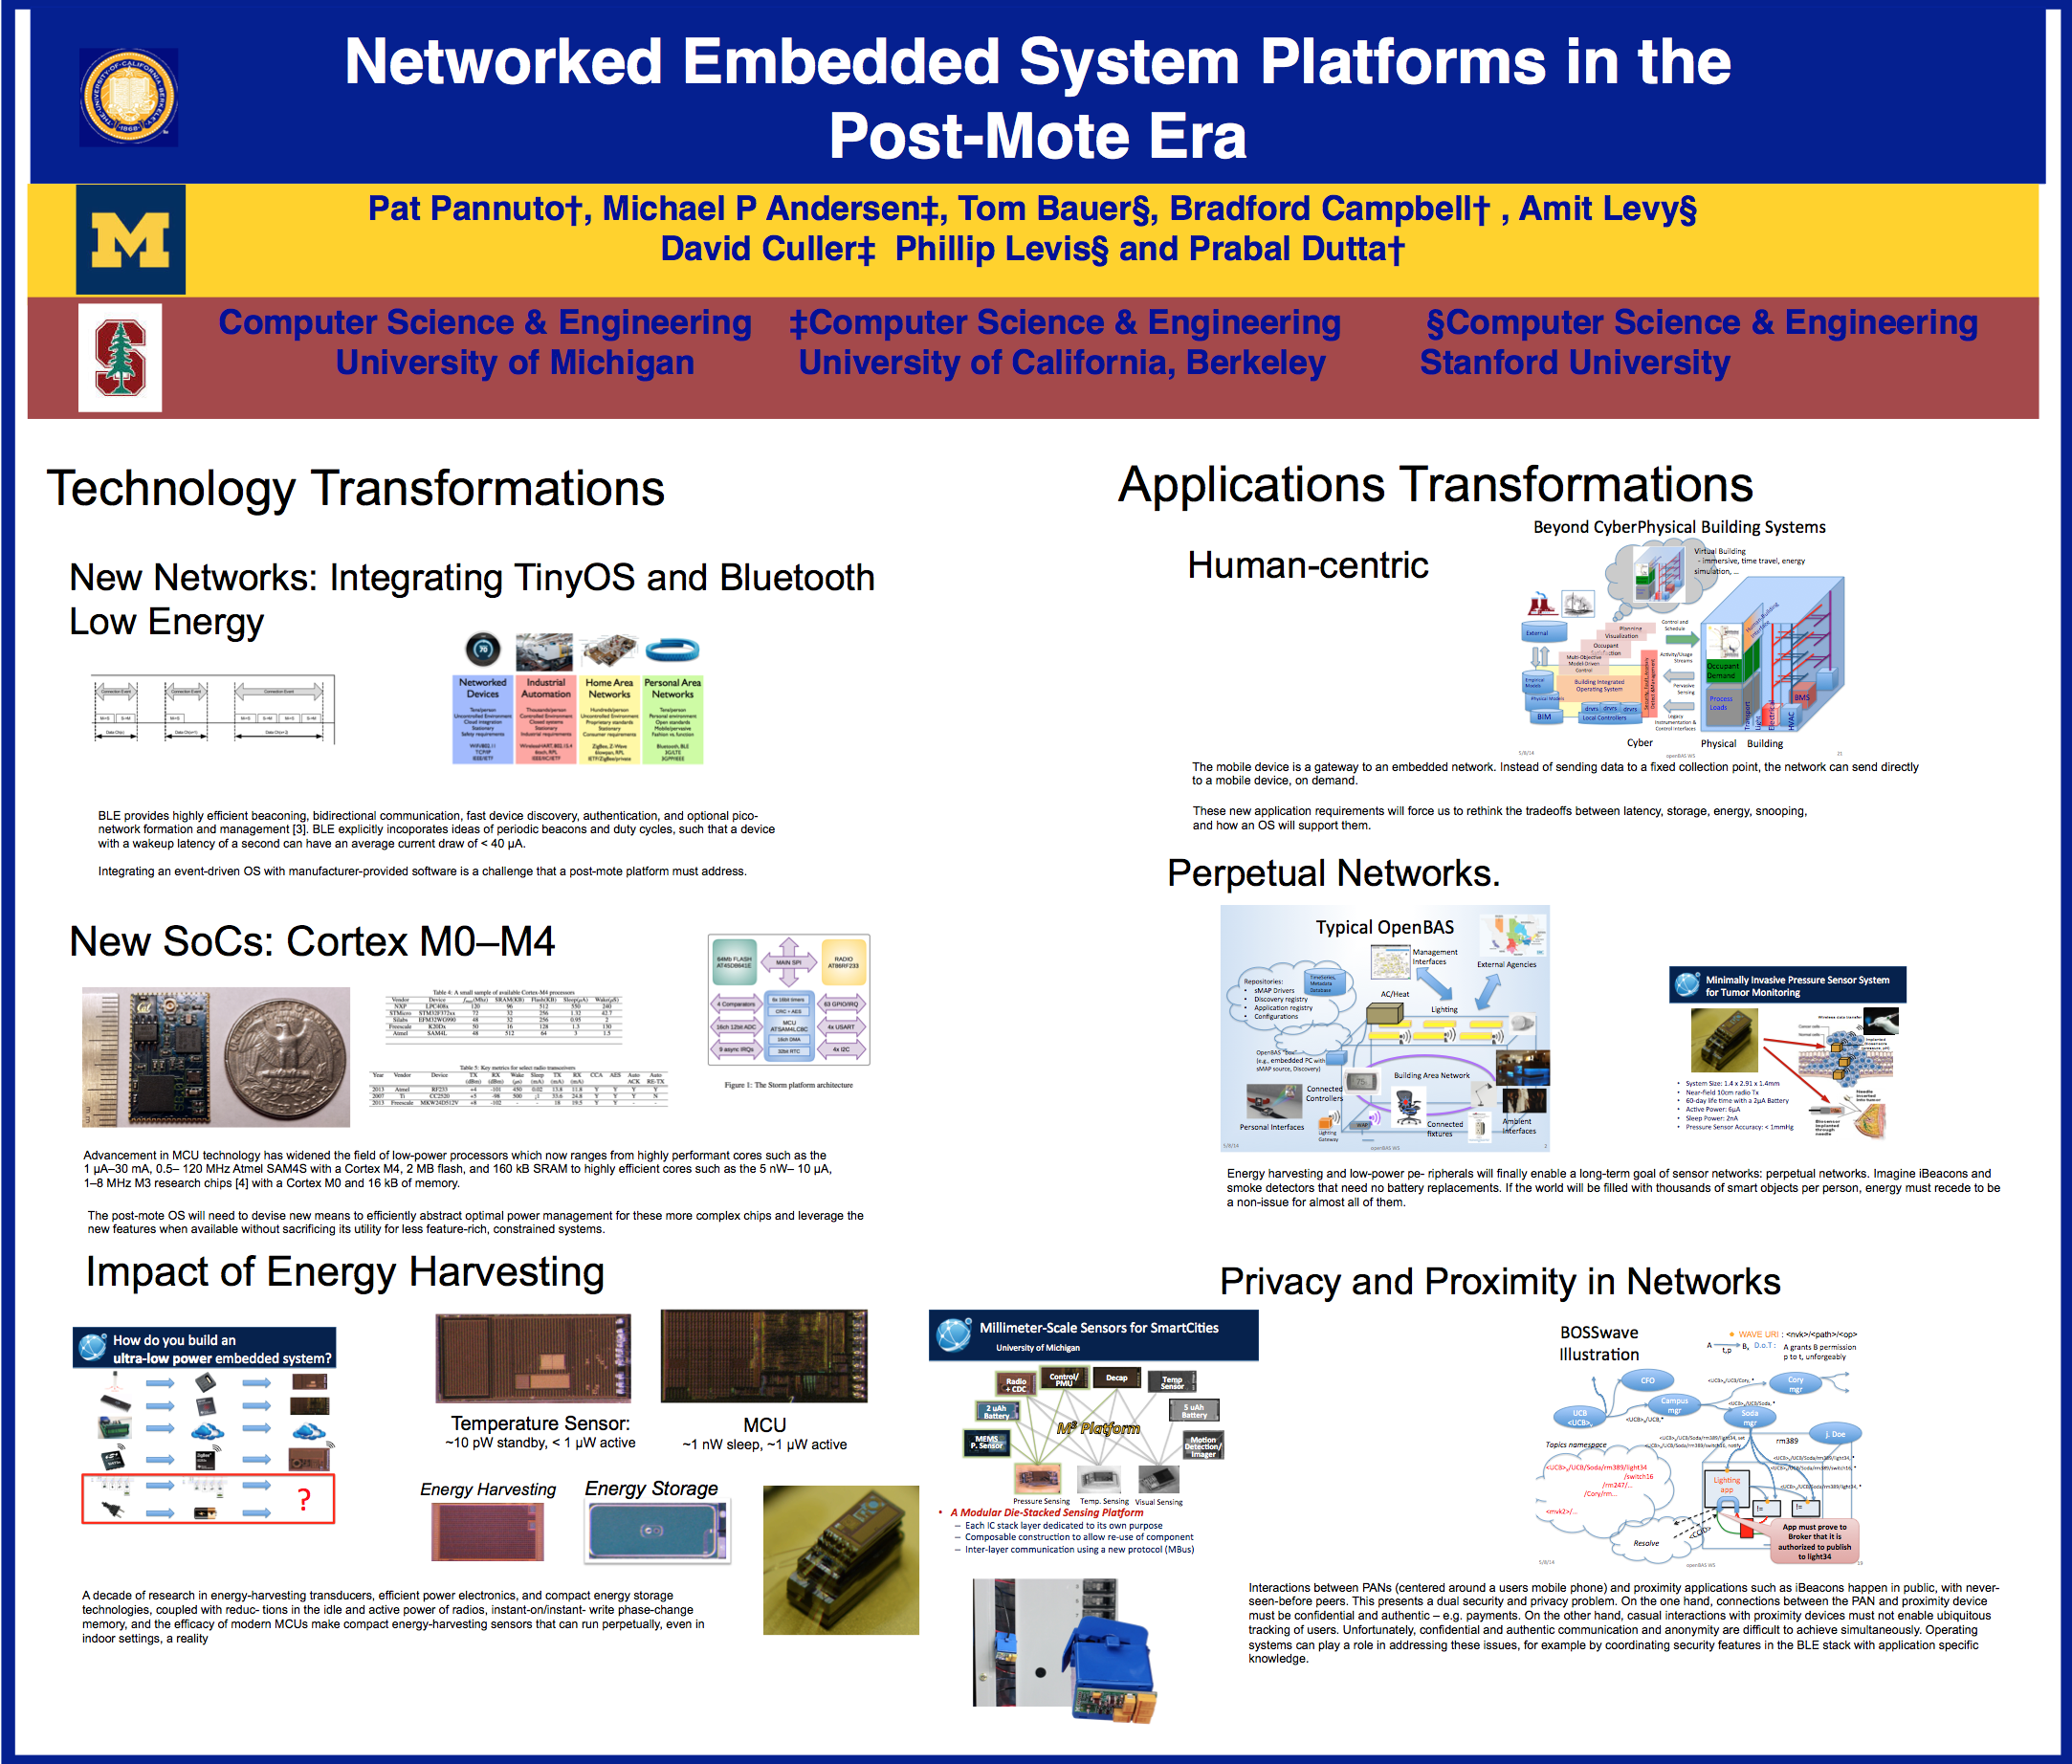
\includegraphics[width=\linewidth]{thumbnail}
%%   \caption{Poster Thumbnail}
%%   \label{fig:poster-thumbnail}
%% \end{figure*}


\end{document}

